\section{Värmeflöde i vägg}

För att beskriva ett värmeflöde används ekvationerna Fouriers värmeekvation
\eqref{eq:staticwallmethod:fourier} och värmeledningsekvationen 
\eqref{eq:staticwallmethod:heat}. 
I dessa är
$k$ värmeledningsförmågan\\i $\mbox{W}\mbox{m}^{-2}\mbox{K}^{-1}$ och
$\alpha$ är termisk diffusivitet i $\mbox{m}^2\mbox{s}^{-1}$. \cite{physicshandbook}

Vid statiskt värmeflöde kommer temperaturderivatan med avseende på tiden att vara noll.
Detta innebär att värmeledningsekvationen övergår i Laplaces ekvation
$\Delta{}T = 0$. I en dimension blir detta $d^2T/dx^2 = 0$ vilket innebär
att lösningen blir ett polynom av första ordningen.  

\begin{equation}
\label{eq:staticwallmethod:fourier}
q_x = -k\frac{dT}{dx}
\end{equation}

\begin{equation}
\label{eq:staticwallmethod:heat}
\frac{\partial{}T}{\partial{}t} = \alpha\Delta{}T
\end{equation}

\begin{figure}
\centering
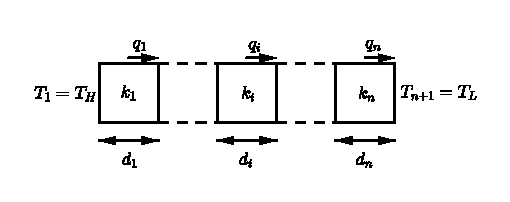
\includegraphics{images/wall.eps}
\caption{Schematisk bild över en vägg som består av $n$ olika element med olika
längd och värmeledningskapacitet.}\label{fig:staticwallmethod:wall}
\end{figure}

\noindent
Vi vill nu beskriva det statiska värmeflödet genom en vägg som består
av flera olika material. De enda värmekällorna som påverkar väggen
är en isoterm $T = T_H$ på ena sidan av väggen
samt en isoterm $T = T_L$ på andra sidan av väggen.

För att göra beräkningarna enklare
ser vi väggen som en oändligt stor skiva. Detta innebär att vi kan räkna
på ekvationen i en dimension. 
En schematisk bild över en vägg i en dimension som består av
$n$ olika material kan ses i figur \ref{fig:staticwallmethod:wall}.
Med materialens värmeledningsförmåga, $k_i$, samt längden
på elementen, $L_i$, använder vi nu Fouriers värmeledningsekvation för
att teckna värmeflödet och temperaturerna $T_j$,  $j=0,\,1,\,...\,,\,n$, i punkterna
mellan de olika delarna av väggen med randvillkoren $T_0 = T_H$ samt
$T_n = T_L$.

För varje del av väggen kan vi sätta upp ekvationer från Fouriers ekvation
för värmeflöde. Vi får flöde in i en del enligt \eqref{eq:staticwallmethod:rod} och
flödet ut genom väggen blir detsamma ty temperaturen är konstant. Dessa två
ekvationer låter oss teckna ett ekvationssystem för varje del av väggen
enligt \eqref{eq:staticwalltheory:rodmatrix}. \cite{lewis04}

\begin{equation}
\label{eq:staticwallmethod:rod}
Q = -k\frac{T_{2}-T_{1}}{L}
\end{equation}


\begin{equation}
\label{eq:staticwalltheory:rodmatrix}
\begin{pmatrix}
Q \\
-Q
\end{pmatrix} = 
\frac{k}{L}\begin{pmatrix}
1 & -1 \\
-1 & 1
\end{pmatrix}
\begin{pmatrix}
T_1 \\
T_2
\end{pmatrix}
\end{equation}

\noindent
Vi kan nu teckna dessa ekvationssystem för alla delar av väggen, som skrivs som 
en matris och sedan fylla ut matriserna med nollelement för att slutligen bilda 
en linjärkomination.
Då linjärkombinationen bildas kommer energiflödena i mitten av väggen att
vara noll. Detta överensstämmer väl med att vi har en statisk energifördelning
utan interna värmekällor.
Slutligen får vi ett ekvationsystem enligt ekvation
\eqref{eq:staticwallmethod:full} som enkelt kan lösas.
Matrisen $A$ är linjärkombinationen av nollutfyllda versioner av matrisen i ekvation
\eqref{eq:staticwalltheory:rodmatrix} enligt ekvation
\eqref{eq:staticwallmethod:example}.

\begin{equation}
\label{eq:staticwallmethod:example}
A = \frac{k_1}{L_1}
\begin{pmatrix}
1 & -1 & 0 &  \dots \\
-1 & 1 & 0 &   \\
0 & 0 & 0 &  \\
\vdots & & & \ddots
\end{pmatrix}
+
\frac{k_2}{L_2}
\begin{pmatrix}
0 & 0 & 0 & 0 & \dots \\
0 & 1 & -1 & 0 &  \\
0 & -1 & 1 & 0 & \\
0 & 0 & 0 & 0 & \\
\vdots & & & & \ddots
\end{pmatrix} + \dots
\end{equation}

\begin{equation}
\label{eq:staticwallmethod:full}
\begin{pmatrix}
Q\\0\\...\\0\\-Q
\end{pmatrix} = A
\begin{pmatrix}
T_H\\T_1\\...\\T_{n-1}\\T_L
\end{pmatrix}
\end{equation}

Här gör vi en jämförelse mellan en oisolerad, 50 cm tjock tegelvägg, motsvarande den som finns på fastighetens södersida, och en 50 cm tjock tegelvägg med 10 cm isolering, motsvarande den som finns på fastighetens norrsida.

\section{Finita element av värmeledningsekvationen}
\label{sec:femheat}
I detta avsnitt behandlas finita elementlösningen av värmeledningsekvationen.
Det är från avsnitt \ref{sec:heatconduction} givet att differentialekvationen
enligt ekvation \eqref{eq:femheateq} beskriver värmeflöde i ett material.

\begin{equation}
\label{eq:femheateq}
c_p\rho\frac{\partial T}{\partial t} = \nabla\cdot(k\nabla T)
\end{equation}

\noindent
För att finna en lösning integreras värmeledningsekvationen
multiplicerat med en $L^2$ integrabel testfunktion $\phi(\mathbf{r})$ över hela
definitionsmängden $\Omega$ vars rand benämns $\Gamma$.
Detta kan ses i ekvation \eqref{eq:femheatweak}.
Nu söks en funktion $T(\mathbf{r},t)$ som satisfierar nyss nämnda uttryck för
alla $L^2$ integrabla testfunktioner $\phi(\mathbf{r})$.

\begin{equation}
\label{eq:femheatweak}
\int_\Omega \left(c_p\rho\frac{\partial T}{\partial t} -
\nabla\cdot(k\nabla T)\right)\phi(\mathbf{r})d\Omega = 0
\end{equation}

\noindent
För att förenkla fortsatta beräkningar behövers det genomföras några
omskrivningar av uttrycket. Divergensteoremet används först för att 
eliminera divergensen i värmeledningsekvationens högerled. Detta ger då
ekvation \eqref{eq:femheatweakfull}. Här är $\mathbf{n}$ normalen till randen.

\begin{equation}
\label{eq:femheatweakfull}
\int_\Omega c_p\rho\frac{\partial T}{\partial t}\phi(\mathbf{r}) +
k\nabla T\nabla\phi(\mathbf{r}) d\Omega =
\int_\Gamma k\mathbf{n}\cdot\nabla Td\Gamma
\end{equation}

\noindent
Härnäst skall galerkinformuleringen skissas. Detta genomförs
genom att temperaturen $T$ samt tidsderivatan av temperaturen $\dot{T}$
enligt ekvationerna \eqref{eq:femheatt} och \eqref{eq:femheattdot}.

\begin{align}
\label{eq:femheatt}
T(\mathbf{r}) & \approx \sum_n T_n\phi(\mathbf{r}) \\
\label{eq:femheattdot}
\dot{T}(\mathbf{r}) & \approx \sum_n \dot{T}_n\phi(\mathbf{r})
\end{align}

\noindent
Ansatsen ovan stoppas härnäst in i den svaga formuleringen i ekvation
\eqref{eq:femheatweakfull} vilket ger ekvation \eqref{eq:femheatgalerkin}.
För att kunna lösa problemet för definitionsmängder som består av olika
homogena material väljs testfunktionen $\phi$ så att den försvinner vid
alla andra material än ett och värmeledningskonstanten kan då benämnas $k_n$.
Ekvationssystemet kan sedan skrivas i matrisform vilket kan ses i ekvation
\eqref{eq:femheatmatrix}. Här är $M$ massmatrisen, $A$ är stelhetsmatrisen och
$f$ är belastningsvektorn.

\begin{align}
\label{eq:femheatgalerkin}
\sum_n \dot{T}_n \int_\Omega c_p\rho\phi_i(\mathbf{r})
\phi_n(\mathbf{r})d\Omega
& + \sum_n T_n \int_\Omega k_n \nabla\phi_n(\mathbf{r})\nabla\phi_n(\mathbf{r})
d\Omega \\
&= \int_\Gamma k_i\phi_i\mathbf{n}\cdot\nabla Td\Gamma \Leftrightarrow
\nonumber
\end{align}

\begin{equation}
\label{eq:femheatmatrix}
M\dot{T} + AT = f \Rightarrow
\end{equation}

\begin{equation}
\label{eq:femheatmatrix2}
\dot{T} + M^{-1}AT = M^{-1}f
\end{equation}

\noindent
Som kan ses så är ovanstående uttryck ett system av kopplade ordinära
differentialekvationer vars lösning är trivial med hjälp av egenvärdesuppdelning.
Vektorerna $\{v\}^n_{i=1}$ definieras som egenvektorerna av
$M^{-1}A$ och $\lambda_i$ definieras som egenvärdena till samma matris.
Systemets homogena lösning kan då skrivas som ekvation
\eqref{eq:femheathom}.\cite{lay06}

\begin{equation}
\label{eq:femheathom}
T_h(t) = \sum_n = c_nv_ne^{-\lambda_nt}
\end{equation}

\noindent
Då ekvationen är inhomogen så återstår det att lösa systemets
partikulärlösning. Då inhomogeniteten är konstant så kan lämpligen
en konstant ansättas som partikulärlösning. Detta ger att
$T_p(t) = D$. Insättning i differentialekvationen ger
ekvation \eqref{eq:femheatinstopp} vilket gör att vi kan bestämma
$D$ genom ekvation \eqref{eq:femheatinstopp2}.

\begin{align}
\label{eq:femheatinstopp}
M^{-1}AD &= M^{-1}b \Rightarrow\\
\label{eq:femheatinstopp2}
D &= A^{-1}b
\end{align}

\noindent
Nu kan den fullständiga lösningen skissas som $T = T_h + T_p$ och om
tiden sätts till noll så kan konstanterna $c_n$ bestämmas genom
att $T$ sätts till problemets begynnelsevärden. För ett problem som
saknar tidsberoende eller som har nått en jämviktspunkt måste
tiden vara oändlig och de termer som innehar exponenter blir noll.
Detta innebär att partikulärlösningen $T_p$ är den tidsoberoende lösningen
till problemet. Detta kan enkelt verifieras genom att sätta $\dot{T} = 0$.
Problemet som återstår är då $AT = b$ vars lösning är $T_p$.

